% Options for packages loaded elsewhere
\PassOptionsToPackage{unicode}{hyperref}
\PassOptionsToPackage{hyphens}{url}
%
\documentclass[
]{article}
\usepackage{lmodern}
\usepackage{amssymb,amsmath}
\usepackage{ifxetex,ifluatex}
\ifnum 0\ifxetex 1\fi\ifluatex 1\fi=0 % if pdftex
  \usepackage[T1]{fontenc}
  \usepackage[utf8]{inputenc}
  \usepackage{textcomp} % provide euro and other symbols
\else % if luatex or xetex
  \usepackage{unicode-math}
  \defaultfontfeatures{Scale=MatchLowercase}
  \defaultfontfeatures[\rmfamily]{Ligatures=TeX,Scale=1}
\fi
% Use upquote if available, for straight quotes in verbatim environments
\IfFileExists{upquote.sty}{\usepackage{upquote}}{}
\IfFileExists{microtype.sty}{% use microtype if available
  \usepackage[]{microtype}
  \UseMicrotypeSet[protrusion]{basicmath} % disable protrusion for tt fonts
}{}
\makeatletter
\@ifundefined{KOMAClassName}{% if non-KOMA class
  \IfFileExists{parskip.sty}{%
    \usepackage{parskip}
  }{% else
    \setlength{\parindent}{0pt}
    \setlength{\parskip}{6pt plus 2pt minus 1pt}}
}{% if KOMA class
  \KOMAoptions{parskip=half}}
\makeatother
\usepackage{xcolor}
\IfFileExists{xurl.sty}{\usepackage{xurl}}{} % add URL line breaks if available
\IfFileExists{bookmark.sty}{\usepackage{bookmark}}{\usepackage{hyperref}}
\hypersetup{
  pdftitle={Fungal metagenomes},
  hidelinks,
  pdfcreator={LaTeX via pandoc}}
\urlstyle{same} % disable monospaced font for URLs
\usepackage[margin=1in]{geometry}
\usepackage{color}
\usepackage{fancyvrb}
\newcommand{\VerbBar}{|}
\newcommand{\VERB}{\Verb[commandchars=\\\{\}]}
\DefineVerbatimEnvironment{Highlighting}{Verbatim}{commandchars=\\\{\}}
% Add ',fontsize=\small' for more characters per line
\usepackage{framed}
\definecolor{shadecolor}{RGB}{248,248,248}
\newenvironment{Shaded}{\begin{snugshade}}{\end{snugshade}}
\newcommand{\AlertTok}[1]{\textcolor[rgb]{0.94,0.16,0.16}{#1}}
\newcommand{\AnnotationTok}[1]{\textcolor[rgb]{0.56,0.35,0.01}{\textbf{\textit{#1}}}}
\newcommand{\AttributeTok}[1]{\textcolor[rgb]{0.77,0.63,0.00}{#1}}
\newcommand{\BaseNTok}[1]{\textcolor[rgb]{0.00,0.00,0.81}{#1}}
\newcommand{\BuiltInTok}[1]{#1}
\newcommand{\CharTok}[1]{\textcolor[rgb]{0.31,0.60,0.02}{#1}}
\newcommand{\CommentTok}[1]{\textcolor[rgb]{0.56,0.35,0.01}{\textit{#1}}}
\newcommand{\CommentVarTok}[1]{\textcolor[rgb]{0.56,0.35,0.01}{\textbf{\textit{#1}}}}
\newcommand{\ConstantTok}[1]{\textcolor[rgb]{0.00,0.00,0.00}{#1}}
\newcommand{\ControlFlowTok}[1]{\textcolor[rgb]{0.13,0.29,0.53}{\textbf{#1}}}
\newcommand{\DataTypeTok}[1]{\textcolor[rgb]{0.13,0.29,0.53}{#1}}
\newcommand{\DecValTok}[1]{\textcolor[rgb]{0.00,0.00,0.81}{#1}}
\newcommand{\DocumentationTok}[1]{\textcolor[rgb]{0.56,0.35,0.01}{\textbf{\textit{#1}}}}
\newcommand{\ErrorTok}[1]{\textcolor[rgb]{0.64,0.00,0.00}{\textbf{#1}}}
\newcommand{\ExtensionTok}[1]{#1}
\newcommand{\FloatTok}[1]{\textcolor[rgb]{0.00,0.00,0.81}{#1}}
\newcommand{\FunctionTok}[1]{\textcolor[rgb]{0.00,0.00,0.00}{#1}}
\newcommand{\ImportTok}[1]{#1}
\newcommand{\InformationTok}[1]{\textcolor[rgb]{0.56,0.35,0.01}{\textbf{\textit{#1}}}}
\newcommand{\KeywordTok}[1]{\textcolor[rgb]{0.13,0.29,0.53}{\textbf{#1}}}
\newcommand{\NormalTok}[1]{#1}
\newcommand{\OperatorTok}[1]{\textcolor[rgb]{0.81,0.36,0.00}{\textbf{#1}}}
\newcommand{\OtherTok}[1]{\textcolor[rgb]{0.56,0.35,0.01}{#1}}
\newcommand{\PreprocessorTok}[1]{\textcolor[rgb]{0.56,0.35,0.01}{\textit{#1}}}
\newcommand{\RegionMarkerTok}[1]{#1}
\newcommand{\SpecialCharTok}[1]{\textcolor[rgb]{0.00,0.00,0.00}{#1}}
\newcommand{\SpecialStringTok}[1]{\textcolor[rgb]{0.31,0.60,0.02}{#1}}
\newcommand{\StringTok}[1]{\textcolor[rgb]{0.31,0.60,0.02}{#1}}
\newcommand{\VariableTok}[1]{\textcolor[rgb]{0.00,0.00,0.00}{#1}}
\newcommand{\VerbatimStringTok}[1]{\textcolor[rgb]{0.31,0.60,0.02}{#1}}
\newcommand{\WarningTok}[1]{\textcolor[rgb]{0.56,0.35,0.01}{\textbf{\textit{#1}}}}
\usepackage{graphicx,grffile}
\makeatletter
\def\maxwidth{\ifdim\Gin@nat@width>\linewidth\linewidth\else\Gin@nat@width\fi}
\def\maxheight{\ifdim\Gin@nat@height>\textheight\textheight\else\Gin@nat@height\fi}
\makeatother
% Scale images if necessary, so that they will not overflow the page
% margins by default, and it is still possible to overwrite the defaults
% using explicit options in \includegraphics[width, height, ...]{}
\setkeys{Gin}{width=\maxwidth,height=\maxheight,keepaspectratio}
% Set default figure placement to htbp
\makeatletter
\def\fps@figure{htbp}
\makeatother
\setlength{\emergencystretch}{3em} % prevent overfull lines
\providecommand{\tightlist}{%
  \setlength{\itemsep}{0pt}\setlength{\parskip}{0pt}}
\setcounter{secnumdepth}{-\maxdimen} % remove section numbering
\usepackage{booktabs}
\usepackage{longtable}
\usepackage{array}
\usepackage{multirow}
\usepackage{wrapfig}
\usepackage{float}
\usepackage{colortbl}
\usepackage{pdflscape}
\usepackage{tabu}
\usepackage{threeparttable}
\usepackage{threeparttablex}
\usepackage[normalem]{ulem}
\usepackage{makecell}
\usepackage{xcolor}

\title{Fungal metagenomes}
\author{}
\date{\vspace{-2.5em}}

\begin{document}
\maketitle

{
\setcounter{tocdepth}{2}
\tableofcontents
}
\hypertarget{analysis-and-commands-run}{%
\subsection{Analysis and commands run}\label{analysis-and-commands-run}}

\hypertarget{initial-preparation}{%
\subsubsection{Initial preparation}\label{initial-preparation}}

Upload samples to server:

\begin{Shaded}
\begin{Highlighting}[]
\FunctionTok{rsync}\NormalTok{ --partial --progress W0.tar.bz2 robyn@vulcan.pharmacology.dal.ca:/home/robyn/}
\FunctionTok{rsync}\NormalTok{ --partial --progress W06.tar.bz2 robyn@vulcan.pharmacology.dal.ca:/home/robyn/}
\FunctionTok{rsync}\NormalTok{ --partial --progress W12.tar.bz2 robyn@vulcan.pharmacology.dal.ca:/home/robyn/}
\end{Highlighting}
\end{Shaded}

Unzip and then gzip:

\begin{Shaded}
\begin{Highlighting}[]
\FunctionTok{tar}\NormalTok{ -xf W0.tar.bz2}
\KeywordTok{for} \ExtensionTok{i}\NormalTok{ in W0_samples/*.fastq }\KeywordTok{;} \KeywordTok{do} \FunctionTok{gzip} \VariableTok{$i} \KeywordTok{;} \KeywordTok{done}

\FunctionTok{tar}\NormalTok{ -xf W06.tar.bz2}
\KeywordTok{for} \ExtensionTok{i}\NormalTok{ in W06_samples/*.fastq }\KeywordTok{;} \KeywordTok{do} \FunctionTok{gzip} \VariableTok{$i} \KeywordTok{;} \KeywordTok{done}

\FunctionTok{tar}\NormalTok{ -xf W12.tar.bz2}
\KeywordTok{for} \ExtensionTok{i}\NormalTok{ in W12_samples/*.fastq }\KeywordTok{;} \KeywordTok{do} \FunctionTok{gzip} \VariableTok{$i} \KeywordTok{;} \KeywordTok{done}
\end{Highlighting}
\end{Shaded}

\hypertarget{kneaddata}{%
\subsubsection{Kneaddata}\label{kneaddata}}

\textbf{Commands run:}

\begin{Shaded}
\begin{Highlighting}[]
\ExtensionTok{parallel}\NormalTok{ -j 1 }\StringTok{'kneaddata -i \{\} -o kneaddata_out_W0/ \textbackslash{}}
\StringTok{-db /home/shared/bowtiedb/GRCh38_PhiX --trimmomatic /home/robyn/tools/Trimmomatic-0.39/ \textbackslash{}}
\StringTok{-t 12 --trimmomatic-options "SLIDINGWINDOW:4:20 MINLEN:50" \textbackslash{}}
\StringTok{--bowtie2-options "--sensitive --dovetail" --remove-intermediate-output'}\NormalTok{ \textbackslash{}}
\NormalTok{ ::: W0_samples/*.fastq.gz}
 \ExtensionTok{kneaddata_read_count_table}\NormalTok{ --input kneaddata_out_W0 --output W0_kneaddata_read_counts.txt}
 \FunctionTok{mkdir}\NormalTok{ W0_decontaminated}
 \KeywordTok{for} \ExtensionTok{i}\NormalTok{ in kneaddata_out_W0/*kneaddata.fastq }\KeywordTok{;} \KeywordTok{do} \FunctionTok{mv} \VariableTok{$i}\NormalTok{ W0_decontaminated }\KeywordTok{;} \KeywordTok{done}
 
 \ExtensionTok{parallel}\NormalTok{ -j 1 }\StringTok{'kneaddata -i \{\} -o kneaddata_out_W06/ \textbackslash{}}
\StringTok{-db /home/shared/bowtiedb/GRCh38_PhiX --trimmomatic /home/robyn/tools/Trimmomatic-0.39/ \textbackslash{}}
\StringTok{-t 12 --trimmomatic-options "SLIDINGWINDOW:4:20 MINLEN:50" \textbackslash{}}
\StringTok{--bowtie2-options "--sensitive --dovetail" --remove-intermediate-output'}\NormalTok{ \textbackslash{}}
\NormalTok{ ::: W06_samples/*.fastq.gz}
 \ExtensionTok{kneaddata_read_count_table}\NormalTok{ --input kneaddata_out_W06 --output W06_kneaddata_read_counts.txt}
 \FunctionTok{mkdir}\NormalTok{ W06_decontaminated}
 \KeywordTok{for} \ExtensionTok{i}\NormalTok{ in kneaddata_out_W06/*kneaddata.fastq }\KeywordTok{;} \KeywordTok{do} \FunctionTok{mv} \VariableTok{$i}\NormalTok{ W06_decontaminated }\KeywordTok{;} \KeywordTok{done}
 
 \ExtensionTok{parallel}\NormalTok{ -j 1 }\StringTok{'kneaddata -i \{\} -o kneaddata_out_W06/ \textbackslash{}}
\StringTok{-db /home/shared/bowtiedb/GRCh38_PhiX --trimmomatic /home/robyn/tools/Trimmomatic-0.39/ \textbackslash{}}
\StringTok{-t 12 --trimmomatic-options "SLIDINGWINDOW:4:20 MINLEN:50" \textbackslash{}}
\StringTok{--bowtie2-options "--sensitive --dovetail" --remove-intermediate-output'}\NormalTok{ \textbackslash{}}
\NormalTok{ ::: W12_samples/*.fastq.gz}
 \ExtensionTok{kneaddata_read_count_table}\NormalTok{ --input kneaddata_out_W12 --output W12_kneaddata_read_counts.txt}
 \FunctionTok{mkdir}\NormalTok{ W12_decontaminated}
 \KeywordTok{for} \ExtensionTok{i}\NormalTok{ in kneaddata_out_W12/*kneaddata.fastq }\KeywordTok{;} \KeywordTok{do} \FunctionTok{mv} \VariableTok{$i}\NormalTok{ W12_decontaminated }\KeywordTok{;} \KeywordTok{done}
\end{Highlighting}
\end{Shaded}

\textbf{W0 percent reads kept:}
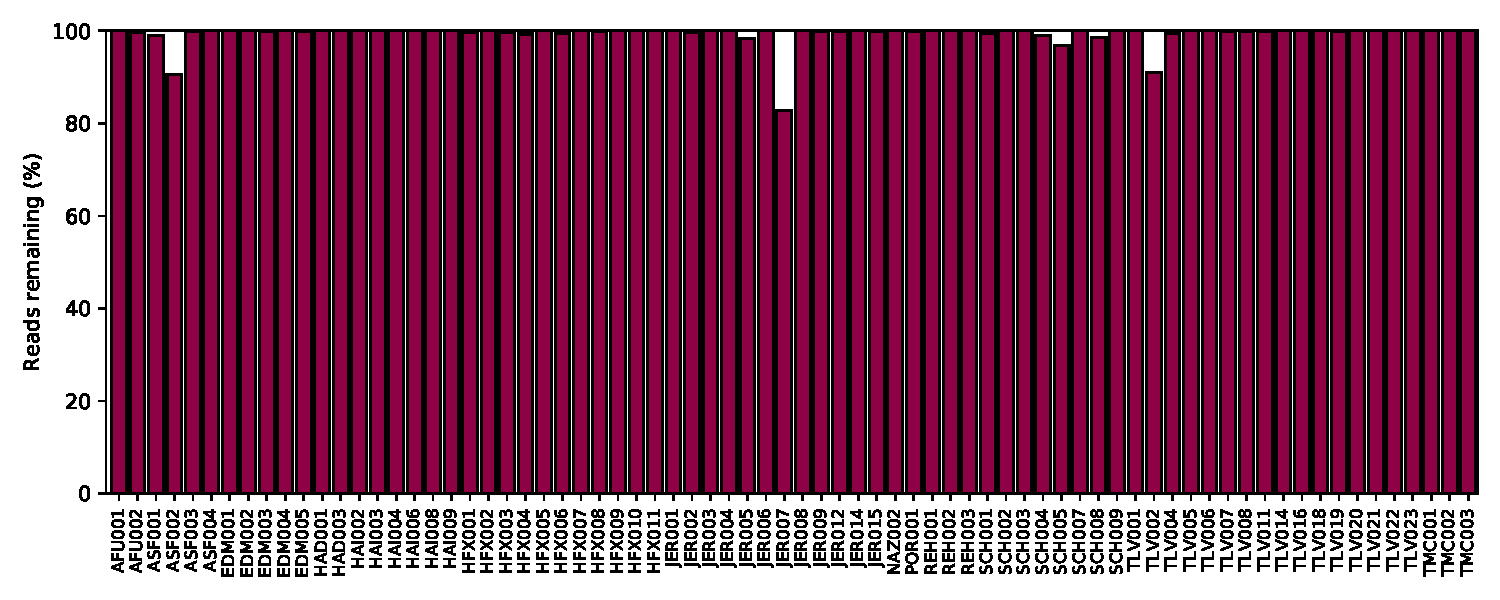
\includegraphics{Fungal-metagenome_files/figure-latex/w0_kneaddata-1.pdf}

\textbf{W06 percent reads kept:}
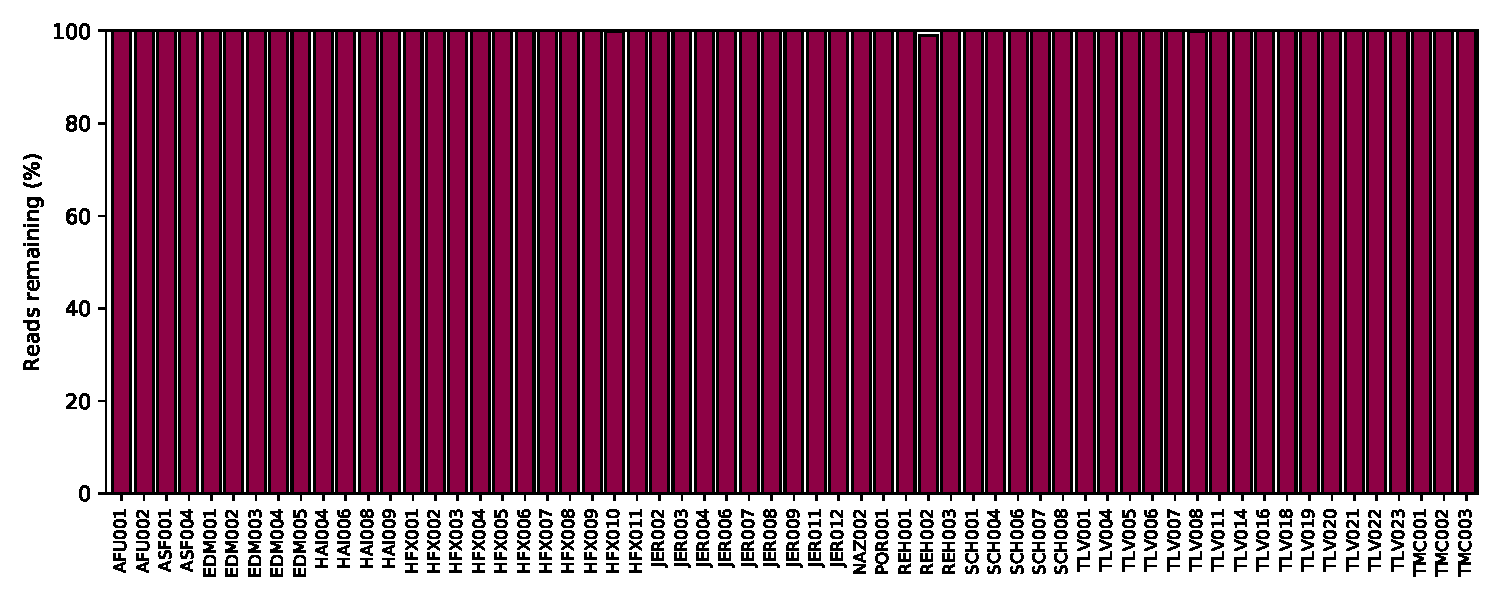
\includegraphics{Fungal-metagenome_files/figure-latex/w06_kneaddata-1.pdf}

\textbf{W12 percent reads kept:}

\hypertarget{kraken2-and-bracken}{%
\subsubsection{Kraken2 and Bracken}\label{kraken2-and-bracken}}

\textbf{Run with RefSeq Complete v93:}

\begin{Shaded}
\begin{Highlighting}[]
\FunctionTok{sudo}\NormalTok{ mount -t ramfs none /scratch/ramdisk/}
\FunctionTok{sudo}\NormalTok{ cp -a /home/shared/Kraken2.0.8_Bracken150mer_RefSeqCompleteV93/ /scratch/ramdisk/}
\FunctionTok{mkdir}\NormalTok{ W0_kraken2_out}
\FunctionTok{mkdir}\NormalTok{ W0_kraken2_kreport}
\ExtensionTok{parallel}\NormalTok{ -j 1 }\StringTok{'kraken2 --use-names --threads 12 --db /scratch/ramdisk/Kraken2.0.8_Bracken150mer_RefSeqCompleteV93/ --memory-mapping \{\} --output W0_kraken2_out/\{/.\}.kraken.txt --report W0_kraken2_kreport/\{/.\}.kreport --confidence 0.1'}\NormalTok{ ::: W0_decontaminated/*.fastq}

\ExtensionTok{parallel}\NormalTok{ -j 1 }\StringTok{'bracken -d /scratch/ramdisk/Kraken2.0.8_Bracken150mer_RefSeqCompleteV93/ -i \{\} -l S -o \{.\}.bracken -r 150'}\NormalTok{ ::: W0_kraken2_kreport/*.kreport}
\end{Highlighting}
\end{Shaded}

\textbf{W0 domain level:}
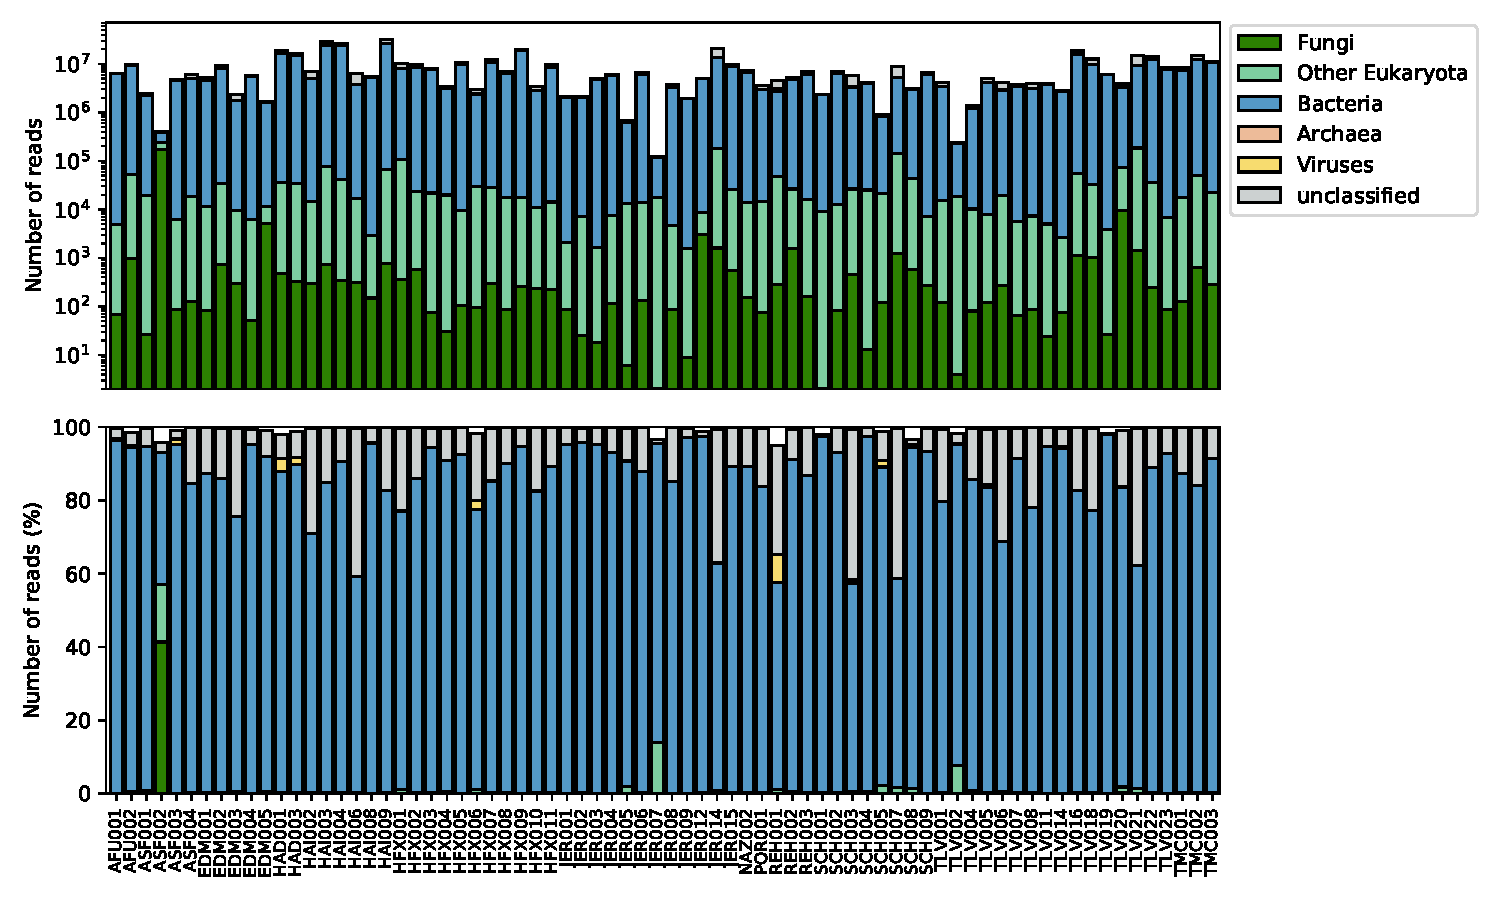
\includegraphics{Fungal-metagenome_files/figure-latex/W0_domain-1.pdf}

\textbf{W06 domain level:}

\textbf{W12 domain level:}

\hypertarget{get-fungal-reads}{%
\subsubsection{Get fungal reads}\label{get-fungal-reads}}

Using
\href{https://github.com/jenniferlu717/KrakenTools.git}{KrakenTools} -
this searches based on the NCBI fungal taxon ID
(\href{https://www.ncbi.nlm.nih.gov/Taxonomy/Browser/wwwtax.cgi?id=4751\&lvl=0}{4751})
and then also takes all lower classifications (because we have used the
--include-children).

\begin{Shaded}
\begin{Highlighting}[]
\FunctionTok{git}\NormalTok{ clone https://github.com/jenniferlu717/KrakenTools.git}

\BuiltInTok{cd}\NormalTok{ W0_kraken2_out}
\KeywordTok{for} \ExtensionTok{i}\NormalTok{ in * }\KeywordTok{;} \KeywordTok{do} \FunctionTok{mv} \VariableTok{$i} \VariableTok{$\{i%}\NormalTok{.*}\VariableTok{\}} \KeywordTok{;} \KeywordTok{done}
\BuiltInTok{cd}\NormalTok{ ..}
\ExtensionTok{parallel}\NormalTok{ -j 1 }\StringTok{'python KrakenTools/extract_kraken_reads.py -k \{\} -s W0_decontaminated/\{/.\}.fastq -o W0_fungi/\{/.\}.fastq -t 4751 --include-children -r W0_kraken2_kreport/\{/.\}.kreport'}\NormalTok{ ::: W0_kraken2_out/*.kraken}
\end{Highlighting}
\end{Shaded}

\hypertarget{humann3}{%
\subsubsection{HUMAnN3}\label{humann3}}

\textbf{Run using Uniref90 and Uniref50 databases:}

\begin{Shaded}
\begin{Highlighting}[]

\end{Highlighting}
\end{Shaded}

\textbf{Combine output files:}

\begin{Shaded}
\begin{Highlighting}[]

\end{Highlighting}
\end{Shaded}

\textbf{Renormalise output files:}

\begin{Shaded}
\begin{Highlighting}[]

\end{Highlighting}
\end{Shaded}

\textbf{Regroup output to other functional categories:}

\begin{Shaded}
\begin{Highlighting}[]

\end{Highlighting}
\end{Shaded}

\hypertarget{taxonomic-analysis}{%
\subsection{Taxonomic analysis}\label{taxonomic-analysis}}

\hypertarget{nmds-plots-all-taxa}{%
\subsubsection{NMDS plots (all taxa)}\label{nmds-plots-all-taxa}}

\hypertarget{nmds-plots-fungi-only}{%
\subsubsection{NMDS plots (fungi only)}\label{nmds-plots-fungi-only}}

\hypertarget{stacked-bar-fungi-genus}{%
\subsubsection{Stacked bar fungi
(genus)}\label{stacked-bar-fungi-genus}}

This is all genera that are above 1\% abundance in at least one sample.
Note that these colours are not unique, but are cycled and the genera
are plotted in order, so as e.g.~Amorphotheca (where present) is plotted
at 0.

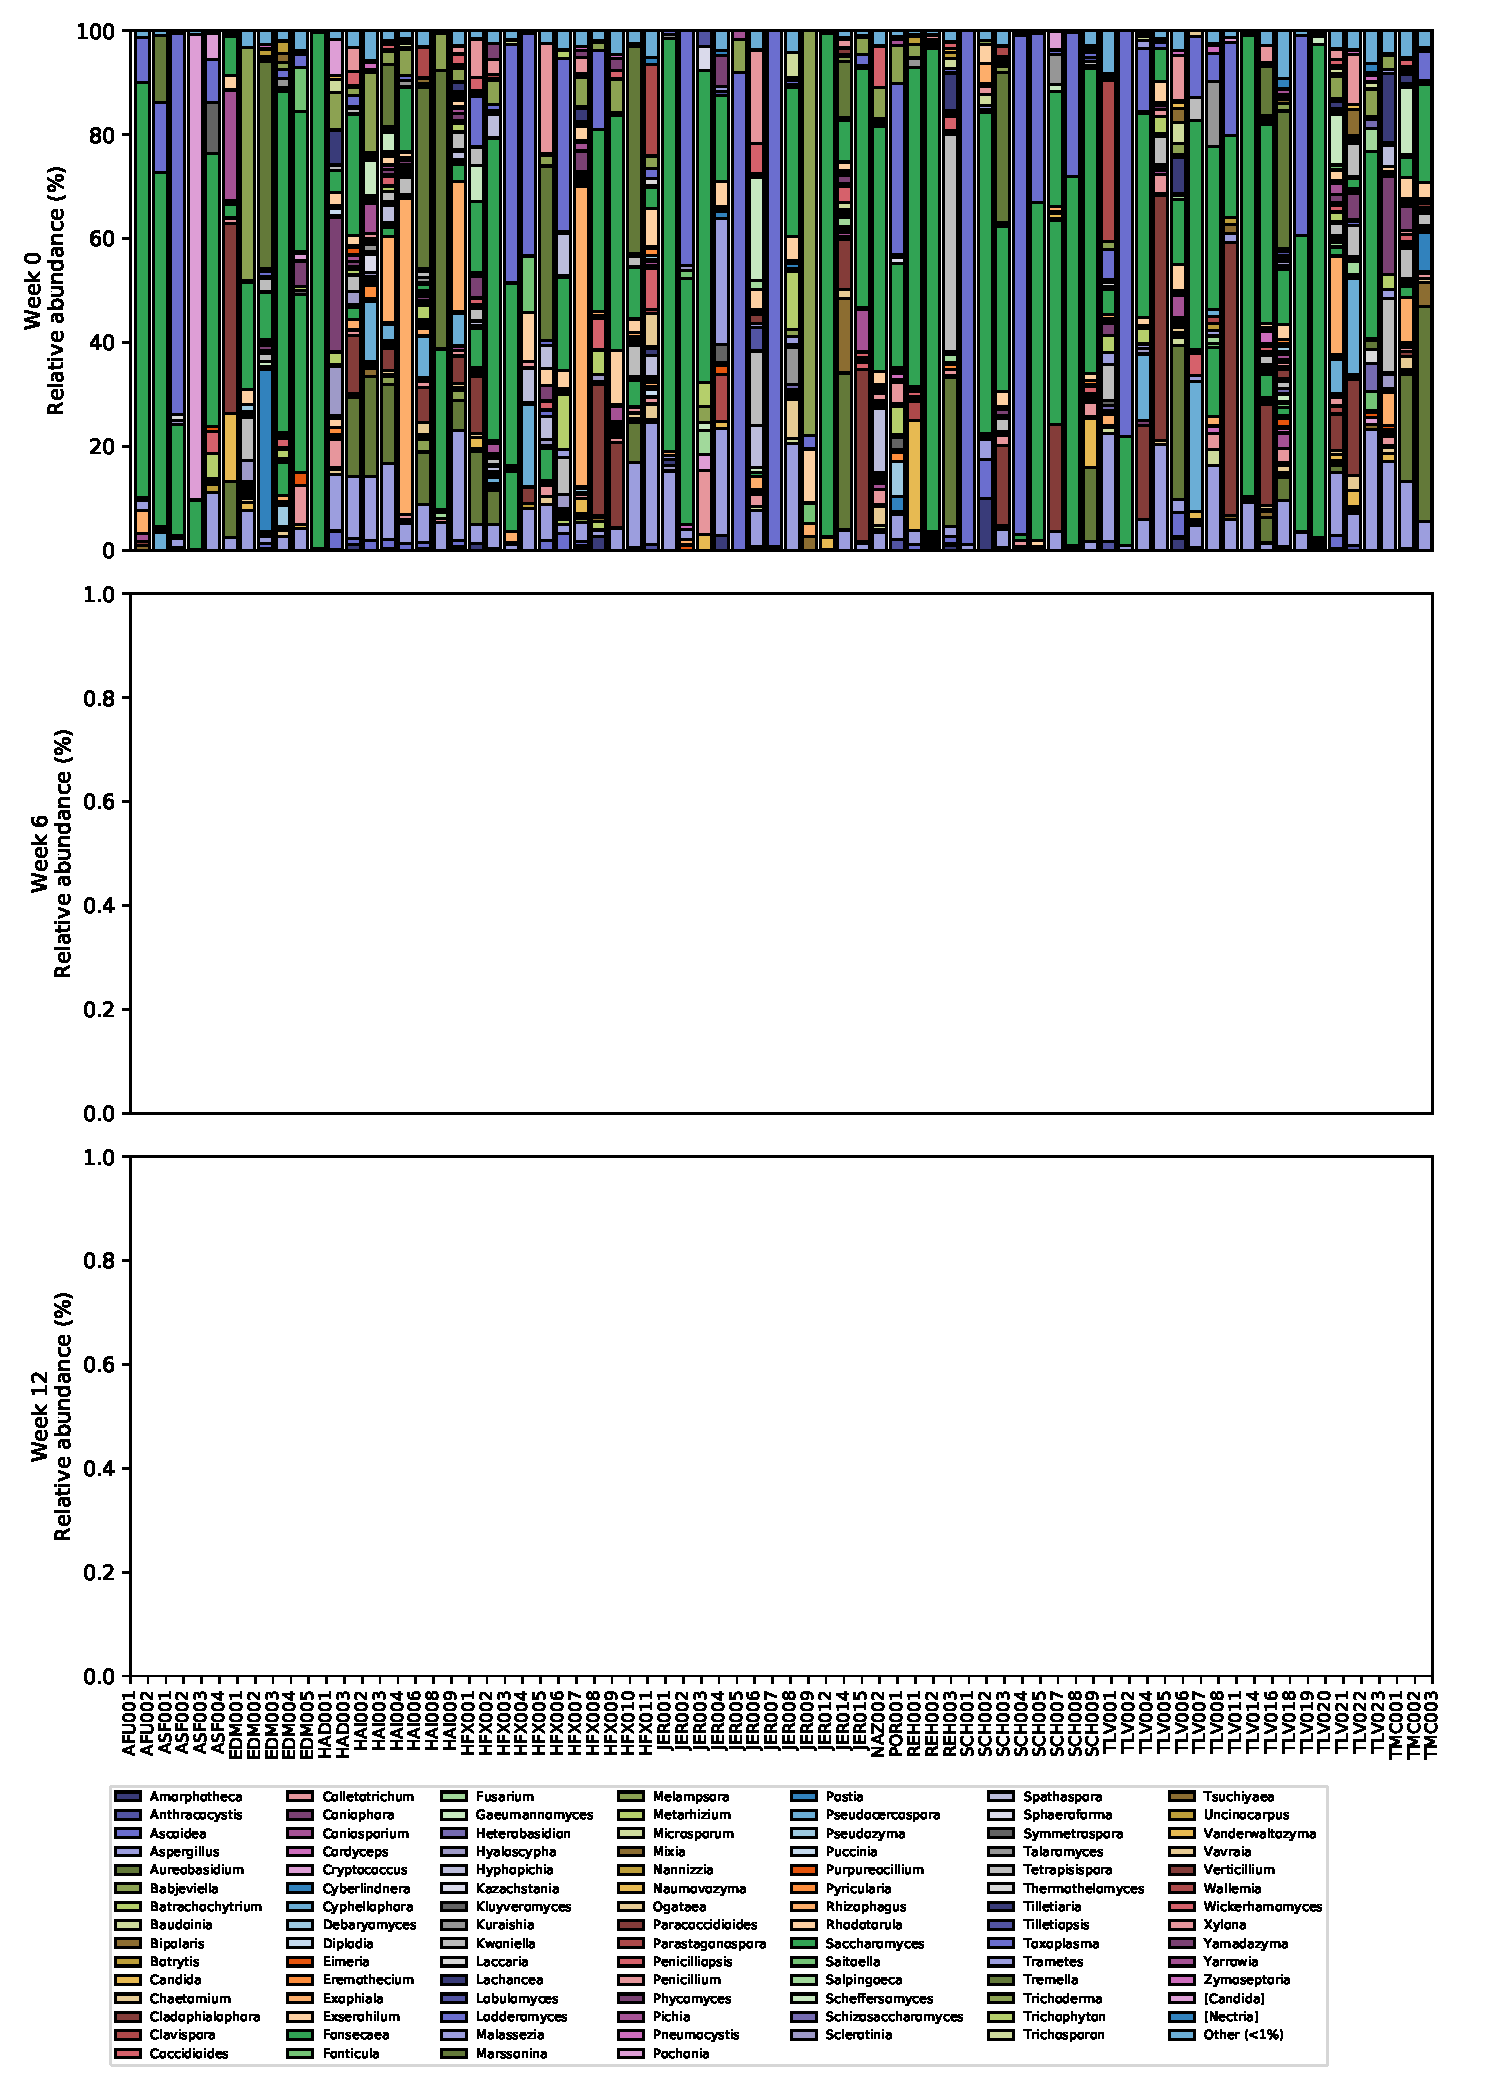
\includegraphics{Fungal-metagenome_files/figure-latex/all_genus-1.pdf}

\hypertarget{functional-analysis}{%
\subsection{Functional analysis}\label{functional-analysis}}

\hypertarget{nmds-plots}{%
\subsubsection{NMDS plots}\label{nmds-plots}}

\hypertarget{gene-family-richness}{%
\subsubsection{Gene family richness}\label{gene-family-richness}}

\hypertarget{pathway-richness}{%
\subsubsection{Pathway richness}\label{pathway-richness}}

\end{document}
